%! Author = drakanoy
%! Date = 10.09.2024

% Preamble
\documentclass[12pt]{article}

% Packages
\usepackage[utf8]{inputenc}
\usepackage[T2A]{fontenc}
\usepackage[english, russian]{babel}
\usepackage[a4paper, includefoot, left=1.5cm, right=1.5cm, top=1cm, bottom=1.5cm, headsep=1cm, footskip=1cm]{geometry}
\usepackage{makecell}
\usepackage{amsmath}
\usepackage{graphicx}
\usepackage{enumitem}
\usepackage{svg}
\usepackage{multirow}
\usepackage{hyperref}
\usepackage{mathtools}
\usepackage{amssymb}
\usepackage{textcomp}

% Document
\begin{document}
\begin{large}
\begin{center}
\LARGE \textbf{Домашняя работа}
\par
\LARGE \textbf{Кононов Александр Михайлович}
\par
    \textbf{25.09.2024}
\end{center}
\par Условие:
\par
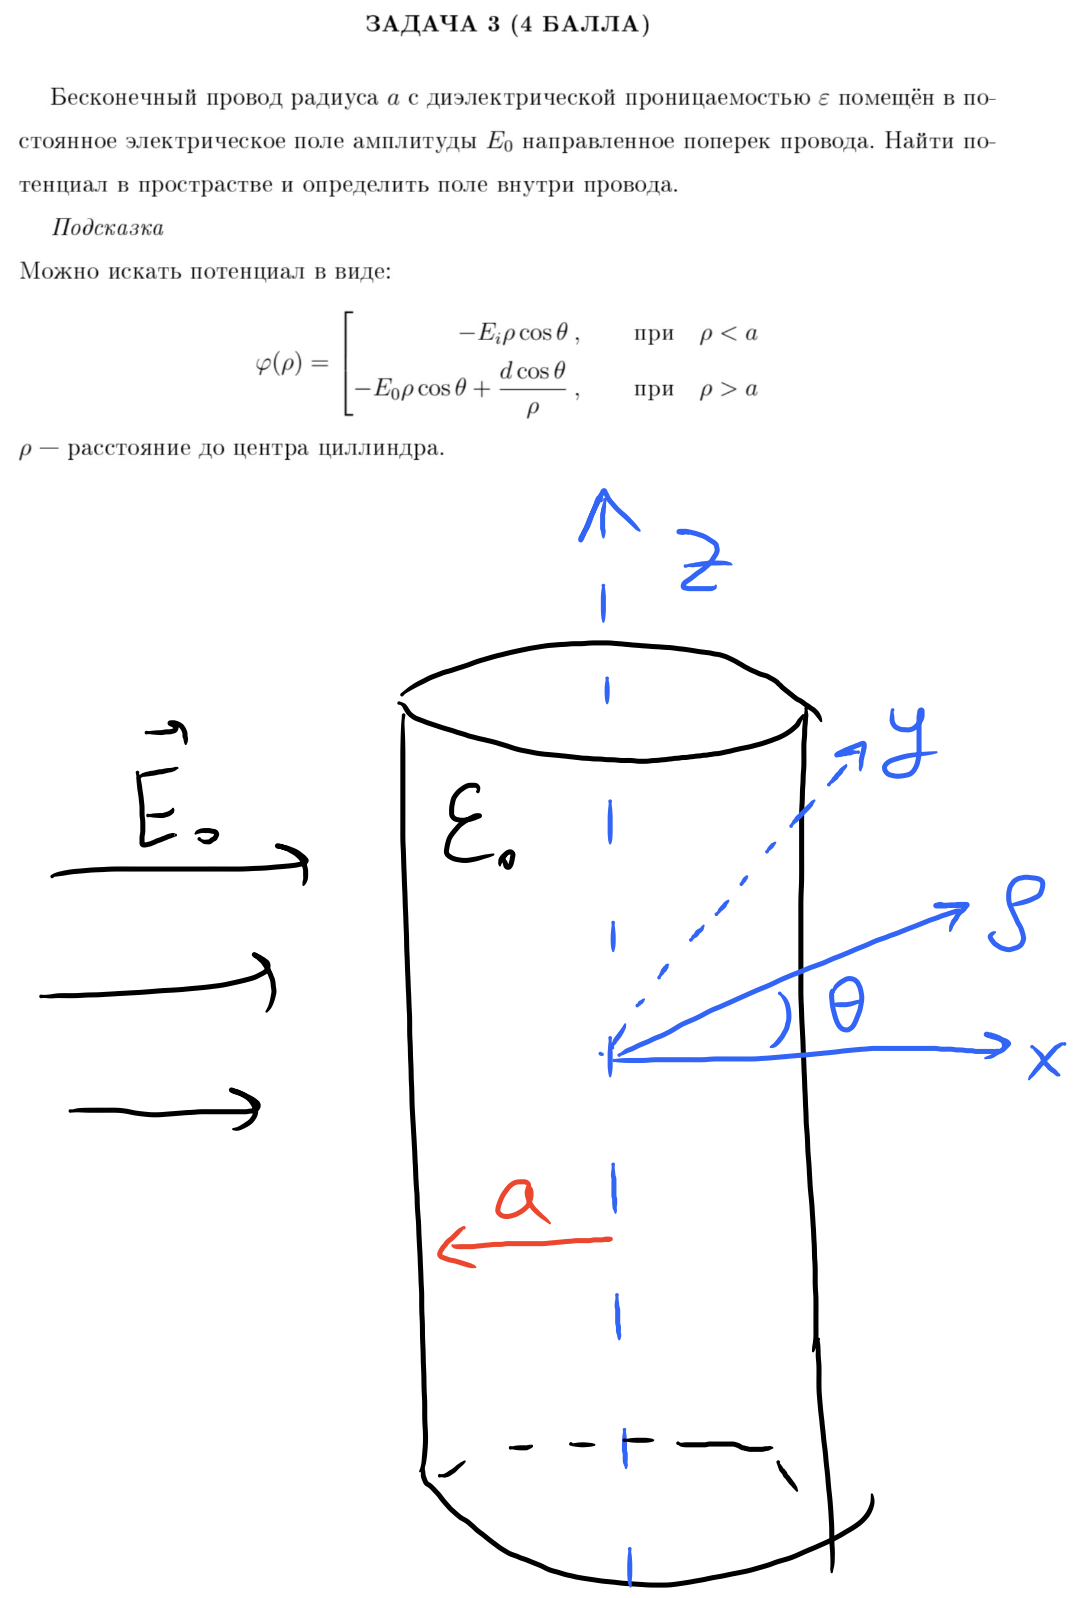
\includegraphics[width=1\textwidth]{photo.png}
%\begin{center}
%\underline{Рисунок 1}:
%\end{center}
\par Решение:
\par Полный потенциал $\varphi$ на $ z = 0 $ является суммой потенциала от точечного заряда $\varphi_0$ и индуцированного потенциала $\varphi_{\text{ind}}$ от поляризации слоя:
\[
    \varphi(\vec{\rho}, z = 0) = \varphi_0(\vec{\rho}, z = 0) + \varphi_{\text{ind}}(\vec{\rho}, z = 0)
\]
\[
    \varphi_0(\vec{\rho}, z = 0) = \frac{e}{\rho}
\]
\par Индуцированная поверхностная плотность заряда $ \sigma_{\text{ind}} $ связана с поляризацией следующим образом:
\[
    \sigma_{\text{ind}}(\vec{\rho}, z) = -\nabla_{\vec{\rho}} \cdot \mathbf{P}_{\parallel}(\vec{\rho}, z)
\]
\par Подставляя
\[
    \mathbf{P}_{\parallel}(\vec{\rho}, z) = \alpha \delta(z) \mathbf{E}_{\parallel}(\vec{\rho})
\]
\par и
\[
    \mathbf{E}_{\parallel}(\vec{\rho}) = -\nabla_{\vec{\rho}} \, \varphi(\vec{\rho}, z = 0)
\]
\par получаем:
\[
    \sigma_{\text{ind}}(\vec{\rho}, z) = \alpha \delta(z) \nabla_{\vec{\rho}}^2 \, \varphi(\vec{\rho}, z = 0)
\]
\par
\[
    \varphi_{\text{ind}}(\vec{\rho}, z) = \int \frac{\sigma_{\text{ind}}(\vec{\rho}\,')}{|\vec{\rho} - \vec{\rho}\,'|} \, d^2 \rho' \delta(z - z') dz' =
\]
\[
    = \int \frac{\sigma_{\text{ind}}(\vec{\rho}')}{|\vec{\rho} - \vec{\rho}\,'|} \, d^2 \rho'
\]
\par Фурье:
\[
    \tilde{f}(\vec{k}, \chi) = \int e^{-i \vec{k} \cdot \vec{\rho} - i z \chi} f(\vec{\rho}, z) \, d^2 \rho dz
\]
\[
    f(\vec{\rho}, z) = \frac{1}{(2\pi)^3} \int e^{i \vec{k} \cdot \vec{\rho} + i z \chi} \tilde{f}(\vec{k}, \chi) \, d^2 k d \chi
\]

\par Для точечного заряда знаем:
\[
    \tilde{\varphi}_0(\vec{k}, \chi) = \int e^{-i \vec{k} \cdot \vec{\rho}} \frac{e}{\rho} \, d^2 \rho = 2\pi \frac{e}{k}
\]
\par Из интегрального представления для индуцироного потенциала получаем уравнение на Фурье образы. Так как под интегралом стоит свертка, то:
\[
    \tilde{\varphi}_{\text{ind}}(\vec{k}, \chi) = 2\pi \frac{\tilde{\sigma}_{\text{ind}}(\vec{k}, \chi)}{k}
\]
\par Используя:
\[
    \sigma_{\text{ind}}(\vec{\rho}) = \alpha \delta(z) \nabla_{\vec{\rho}}^2 \, \varphi(\vec{\rho}, z = 0)
\]
\par получаем:
\[
\tilde{\sigma}_{\text{ind}}(\vec{k}, \chi) = -\alpha k^2 \tilde{\varphi}(\vec{k}, \chi)
\]
\par Подставляем:
\[
    \tilde{\varphi}_{\text{ind}}(\vec{k}, \chi) = -2\pi \alpha k \tilde{\varphi}(\vec{k}, \chi)
\]
\par Так как:
\[
\tilde{\varphi}(\vec{k}, \chi) = \tilde{\varphi}_0(\vec{k}), \chi + \tilde{\varphi}_{\text{ind}}(\vec{k}, \chi) = \tilde{\varphi}_0(\vec{k}, \chi) - 2\pi \alpha k \tilde{\varphi}(\vec{k}, \chi)
\]
\[
\left(1 + 2\pi \alpha k\right) \tilde{\varphi}(\vec{k}, \chi) = 2\pi \frac{e}{k}
\]
\[
\tilde{\varphi}(\vec{k}, \chi) = \frac{2\pi e}{k \left(1 + 2\pi \alpha k\right)}
\]

\par Обратный Фурье:
\par По $z = 0$ ничего не меняется:
\[
    \tilde{\varphi}(\vec{k}, z = 0) = \frac{2\pi e}{k \left(1 + 2\pi \alpha k\right)}
\]
\[
    \varphi(\vec{\rho}, z = 0) = \int \frac{d^2 k}{(2\pi)^2} \cdot e^{i \vec{k} \cdot \vec{\rho}} \cdot \frac{2\pi e}{k \left(1 + 2\pi \alpha k\right)} =
\]
\[
    = \int\limits_0^{ \infty} \int\limits_0^{ 2\pi} \frac{k dk d \theta}{(2\pi)^2} \cdot e^{i k \rho \cos(\theta)} \cdot \frac{2\pi e}{k \left(1 + 2\pi \alpha k\right)} =
\]
\[
    = \int\limits_0^{ \infty} \frac{dk}{2\pi} \cdot \frac{2\pi e}{\left(1 + 2\pi \alpha k\right)} \int\limits_0^{ 2\pi} \frac{d \theta}{2\pi} \cdot e^{i k \rho \cos(\theta)}
\]
\[
    = \int\limits_0^{ \infty} \frac{dk}{2\pi} \cdot \frac{2\pi e}{\left(1 + 2\pi \alpha k\right)} \cdot J_0(k \rho) =
\]
\[
    = \frac{2\pi e}{4 \pi^2 \alpha} \int\limits_0^{ \infty} dx \frac{J_0(x \cdot \rho/2\pi\alpha)}{1 + x}
\]
\[
    = \frac{e}{4\alpha} \left[ H_0(\rho/2\pi\alpha) - N_0(\rho/2\pi\alpha) \right]
\]
\par Ответ:
\[
    \varphi(\vec{\rho}, z = 0) = \frac{e}{4\alpha} \left[ H_0(\rho/2\pi\alpha) - N_0(\rho/2\pi\alpha) \right]
\]
\end{large}
\end{document}
